\section{講義概要}


\begin{frame}
\frametitle{今日の内容}



\begin{enumerate}
\item 三角関数, 指数関数, 対数関数の微分,
\item 合成関数の微分, 対数微分
\end{enumerate} 



\end{frame}





%%%%%%%%%%%%%%%%%%%%%%%%%%%%%%%%%%%%%%%%%%%%%%%%%%%%%%%%%%%%%%%%%%%%%%%%%%%%%%%%%%%%%%%
%%%%%%%%%%%%%%%%%%%%%%%%%%%%%%%%%%%%%%%%%%%%%%%%%%%%%%%%%%%%%%%%%%%%%%%%%%%%%%%%%%%%%%%

\section{三角関数の微分}

\begin{frame}
\frametitle{三角関数の微分}


\vspace{-4mm}

三角関数の微分を議論するために必要な準備を行う. 

\vspace{-1mm}

\begin{Thm} \label{準備}
\begin{enumerate}
\item $\displaystyle\lim_{x \to 0} \frac{\sin x}{x}=1$, 
\item  $\displaystyle \lim_{x \to 0} \frac{1-\cos x}{x}=0$. 
\end{enumerate}
\end{Thm}
弧度法において, $x$が弧の長さであることから$0<x<\pi/2$において次の不等式が成立する. 
(扇形と底辺を共有する2つの三角形の面積を比較しても良い.)
\vspace{-6mm}

 \begin{figure}[htbp]
 \begin{center} 
  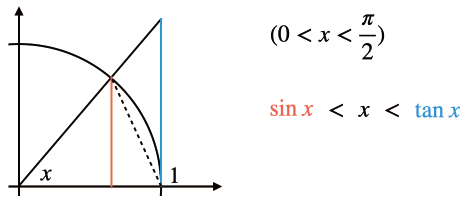
\includegraphics[width=65mm]{calculus5/sintan.png}
 \end{center}
\end{figure}

\vspace{-10mm}

\end{frame}





%%%%%%%%%%%%%%%%%%%%%%%%%%%%%%%%%%%%%%%%%%%%%%%%%%%%%%%%%%%%%%%%%%%%%%%%%%%%%%%%%%%%%%%
%%%%%%%%%%%%%%%%%%%%%%%%%%%%%%%%%%%%%%%%%%%%%%%%%%%%%%%%%%%%%%%%%%%%%%%%%%%%%%%%%%%%%%%


\begin{frame}
\frametitle{定理\ref{準備}\ctext{1}の証明}

$0<x<\pi/2$において
\begin{itemize}
\item $\sin x < x$より, $\frac{\sin x}{x}<1$. 
\item $x < \tan x=\frac{\sin x}{\cos x}$より, $\cos x < \frac{\sin x}{x}$.   
\end{itemize}
纏めると
$$
\cos x < \frac{\sin x}{x} < 1. 
$$
$x \to +0$なる極限をとると
$$
\lim_{x \to +0} \cos x \le \lim_{x \to +0} \frac{\sin x}{x} \le \lim_{x \to +0} 1. 
$$
これより, $\displaystyle\lim_{x \to +0} \frac{\sin x}{x}=1$. (挟み撃ちの定理)\\
\ \\

同様の議論で左極限も$\displaystyle\lim_{x \to -0} \frac{\sin x}{x}=1$.  

\end{frame}



%%%%%%%%%%%%%%%%%%%%%%%%%%%%%%%%%%%%%%%%%%%%%%%%%%%%%%%%%%%%%%%%%%%%%%%%%%%%%%%%%%%%%%%
%%%%%%%%%%%%%%%%%%%%%%%%%%%%%%%%%%%%%%%%%%%%%%%%%%%%%%%%%%%%%%%%%%%%%%%%%%%%%%%%%%%%%%%


\begin{frame}
\frametitle{定理\ref{準備}\ctext{2}の証明}

$\sin^2x +\cos^2 x=1$より
$$
\frac{1-\cos x}{x}
=
\frac{1-\cos ^2x}{x(1+\cos x)}
=
\frac{\sin ^2x}{x(1+\cos x)}
=
\frac{\sin x}{x}
\frac{\sin x}{1+\cos x}
$$
であるから 
$$
\lim_{x \to 0} \frac{1-\cos x}{x}=
\lim_{x \to 0} (\frac{\sin x}{x}
\frac{\sin x}{1+\cos x})
=1 \cdot \frac{0}{1+1}=0. 
$$

\end{frame}




%%%%%%%%%%%%%%%%%%%%%%%%%%%%%%%%%%%%%%%%%%%%%%%%%%%%%%%%%%%%%%%%%%%%%%%%%%%%%%%%%%%%%%%
%%%%%%%%%%%%%%%%%%%%%%%%%%%%%%%%%%%%%%%%%%%%%%%%%%%%%%%%%%%%%%%%%%%%%%%%%%%%%%%%%%%%%%%


\begin{frame}
\frametitle{三角関数の微分}



\begin{Thm} \label{三角関数微分}
\begin{enumerate}
\item $(\sin x)'=\cos x$,
\item  $(\cos x)' = -\sin x$,
\item $(\tan x)'=\frac{1}{\cos^2 x}$. 
\end{enumerate}
\end{Thm}

三角関数の加法定理を思い出しておく. 
\begin{itemize}
\item $\sin(\alpha+\beta)=\sin \alpha \cos \beta + \cos \alpha \sin \beta$
\item $\cos(\alpha+\beta)=\cos \alpha \cos \beta - \sin \alpha \sin \beta$
\end{itemize}

\end{frame}
\begin{slide}{加法定理の図的な説明}
%\begin{eqnarray}
%\sin(A+B) &=& \sin{A}\cos{B} + \sin{B}\cos{A} \\
%\sin(A-B) &=& \sin{A}\cos{B} - \sin{B}\cos{A} \\
%\cos(A+B) &=& \cos{A}\cos{B}-\sin{A}\sin{B} \\
%\cos(A-B)&=&\cos{A}\cos{B}+\sin{A}\sin{B}
%\end{eqnarray}
\begin{figure}[h]                                                                      
\centering
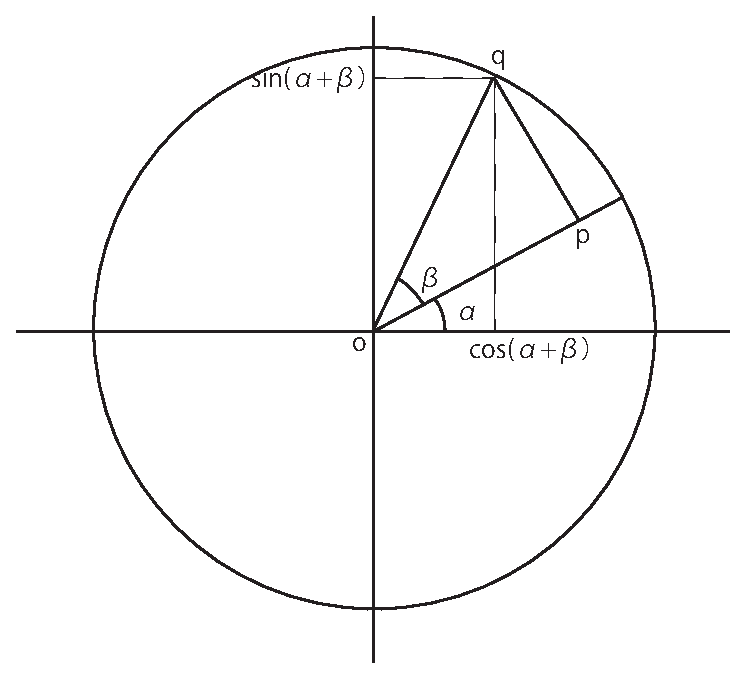
\includegraphics[width=3cm]{calculus5/add.eps}
%\caption{加法定理の図解}
%\label{fig:additive}
\end{figure}
\begin{equation}
\overrightarrow{op} = \cos{\beta}(\cos{\alpha}, \sin{\alpha})
\end{equation}
であり、$\overrightarrow{pq}$は$\overrightarrow{op}$に直交して長さが$\sin{\beta}$であるため
\begin{equation}
\overrightarrow{pq} = \sin{\beta}(-\sin{\alpha}, \cos{\alpha})
\end{equation}
となるため$\overrightarrow{oq}$は
\begin{eqnarray}
\overrightarrow{oq} &=& \overrightarrow{op}+\overrightarrow{pq}\nonumber \\
&=& (\cos{\alpha}\cos{\beta} - \sin{\alpha}\sin{\beta}, \sin{\alpha}\cos{\beta}+\sin{\beta}\cos{\alpha})
\end{eqnarray}
となり、加法定理を与える。
\end{slide}


%%%%%%%%%%%%%%%%%%%%%%%%%%%%%%%%%%%%%%%%%%%%%%%%%%%%%%%%%%%%%%%%%%%%%%%%%%%%%%%%%%%%%%%
%%%%%%%%%%%%%%%%%%%%%%%%%%%%%%%%%%%%%%%%%%%%%%%%%%%%%%%%%%%%%%%%%%%%%%%%%%%%%%%%%%%%%%%


\begin{frame}
\frametitle{定理\ref{三角関数微分}\ctext{1}の証明}

加法定理より
\begin{align*}
\sin(x +h)-\sin x & = \sin x \cos h + \cos x \sin h -\sin x \\
& =  \cos x \sin h + \sin x( \cos h-1)
\end{align*}
であるから
\begin{align*}
(\sin x)' &= \lim_{h \to 0} \frac{\sin(x +h)-\sin x}{h} \\
& =  \lim_{h \to 0} (\cos x \frac{\sin h}{h} + \sin x \frac{\cos h-1}{h}) \\
& =\cos x \cdot 1 + \sin x \cdot 0 \\
& = \cos x. 
\end{align*}
\end{frame}


%%%%%%%%%%%%%%%%%%%%%%%%%%%%%%%%%%%%%%%%%%%%%%%%%%%%%%%%%%%%%%%%%%%%%%%%%%%%%%%%%%%%%%%
%%%%%%%%%%%%%%%%%%%%%%%%%%%%%%%%%%%%%%%%%%%%%%%%%%%%%%%%%%%%%%%%%%%%%%%%%%%%%%%%%%%%%%%


\begin{frame}
\frametitle{定理\ref{三角関数微分}\ctext{2}の証明}

加法定理より
\begin{align*} 
\cos(x +h)-\cos x & = \cos x \cos h - \sin x \sin h -\cos x \\
& =  \cos x (\cos h-1) - \sin x \sin h
\end{align*}
であるから
\begin{align*}
(\cos x)' &= \lim_{h \to 0} \frac{\cos(x +h)-\cos x}{h} \\
& =  \lim_{h \to 0} (\cos x \frac{\cos h-1}{h} - \sin x \frac{\sin h}{h}) \\
& =\cos x \cdot 0 - \sin x \cdot 1 \\
& = -\sin x. 
\end{align*}
\end{frame}


%%%%%%%%%%%%%%%%%%%%%%%%%%%%%%%%%%%%%%%%%%%%%%%%%%%%%%%%%%%%%%%%%%%%%%%%%%%%%%%%%%%%%%%
%%%%%%%%%%%%%%%%%%%%%%%%%%%%%%%%%%%%%%%%%%%%%%%%%%%%%%%%%%%%%%%%%%%%%%%%%%%%%%%%%%%%%%%


\begin{frame}
\frametitle{定理\ref{三角関数微分}\ctext{3}の証明}

商の微分公式より
\begin{align*} 
(\tan x)' &= \Big( \frac{\sin x}{\cos x} \Big)' \\
&= \frac{(\sin x)'\cos x - \sin x (\cos x)'}{\cos^2 x} \\
&= \frac{\cos^2 x + \sin^2 x}{\cos^2 x} \\
&= \frac{1}{\cos^2 x}. 
\end{align*}

\end{frame}


%%%%%%%%%%%%%%%%%%%%%%%%%%%%%%%%%%%%%%%%%%%%%%%%%%%%%%%%%%%%%%%%%%%%%%%%%%%%%%%%%%%%%%%
%%%%%%%%%%%%%%%%%%%%%%%%%%%%%%%%%%%%%%%%%%%%%%%%%%%%%%%%%%%%%%%%%%%%%%%%%%%%%%%%%%%%%%%


\begin{frame}
\frametitle{三角関数の微分}

\begin{Prob}
次の関数の導関数を求めよ. 
\begin{enumerate}
\item $\sin^2 x$
\item $\sin^3 x$
\item $\sin x \cos x$
\item $\frac{\cos x}{x}$
\end{enumerate}
\end{Prob}

\end{frame}


%%%%%%%%%%%%%%%%%%%%%%%%%%%%%%%%%%%%%%%%%%%%%%%%%%%%%%%%%%%%%%%%%%%%%%%%%%%%%%%%%%%%%%%
%%%%%%%%%%%%%%%%%%%%%%%%%%%%%%%%%%%%%%%%%%%%%%%%%%%%%%%%%%%%%%%%%%%%%%%%%%%%%%%%%%%%%%%

\section{指数関数と対数関数の微分}

\begin{frame}
\frametitle{ネイピア数}

ネイピア数$e=2.71828\dots$に関して, 次が成立する.  
$$
e=\lim_{x \to +\infty} \Big(1+\frac{1}{x}\Big)^x = \lim_{x \to -\infty} \Big(1+\frac{1}{x}\Big)^x. 
$$
これは$\displaystyle e=\lim_{x\to 0}(1+x)^\frac{1}{x}$とも同値である. \\
\ \\

いくつか計算してみると
\begin{align*}
(1+\frac{1}{10})^{10}&=2.5937\dots, \ \ \ 
(1+\frac{1}{100})^{100}=2.7048\dots, \\
(1+\frac{1}{1000})^{1000}&=2.7169\dots, \ \ \ 
(1+\frac{1}{10000})^{10000}=2.7181\dots, 
\end{align*}

\end{frame}




%%%%%%%%%%%%%%%%%%%%%%%%%%%%%%%%%%%%%%%%%%%%%%%%%%%%%%%%%%%%%%%%%%%%%%%%%%%%%%%%%%%%%%%
%%%%%%%%%%%%%%%%%%%%%%%%%%%%%%%%%%%%%%%%%%%%%%%%%%%%%%%%%%%%%%%%%%%%%%%%%%%%%%%%%%%%%%%



\begin{frame}
\frametitle{準備}

指数関数と対数関数の微分を議論するために必要な準備を行う. 

\begin{Thm} \label{準備2}
\begin{enumerate}
\item $\displaystyle \lim_{h \to 0} \frac{e^h-1}{h}=1$, 
\item  $\displaystyle \lim_{h \to 0} \frac{\log(1+h)}{h}=1$. 
\end{enumerate}
\end{Thm}


\end{frame}



%%%%%%%%%%%%%%%%%%%%%%%%%%%%%%%%%%%%%%%%%%%%%%%%%%%%%%%%%%%%%%%%%%%%%%%%%%%%%%%%%%%%%%%
%%%%%%%%%%%%%%%%%%%%%%%%%%%%%%%%%%%%%%%%%%%%%%%%%%%%%%%%%%%%%%%%%%%%%%%%%%%%%%%%%%%%%%%


\begin{frame}
\frametitle{定理\ref{準備2}の証明}

まず\ctext{2}を示す. 
\begin{align*} 
\lim_{h \to 0} \frac{\log(1+h)}{h} & = \lim_{h \to 0} \log(1+h)^{\frac{1}{h}} \\
& = \log \big( \lim_{h \to 0} (1+h)^{\frac{1}{h}} \big) \ \ \ (\text{対数関数の連続性})\\
& = \log e = 1. 
\end{align*}
次に\ctext{1}を示す. 
まず$t=e^h-1$とおくと, $h\to 0$のとき$t\to0$である. 
また$e^h=1+t$より$h=\log (1+t)$であるから, \ctext{2}より
$$
\lim_{h \to 0} \frac{e^h-1}{h}=\lim_{t \to 0} \frac{t}{\log(1+t)}=1. 
$$

\end{frame}


%%%%%%%%%%%%%%%%%%%%%%%%%%%%%%%%%%%%%%%%%%%%%%%%%%%%%%%%%%%%%%%%%%%%%%%%%%%%%%%%%%%%%%%
%%%%%%%%%%%%%%%%%%%%%%%%%%%%%%%%%%%%%%%%%%%%%%%%%%%%%%%%%%%%%%%%%%%%%%%%%%%%%%%%%%%%%%%


\begin{frame}
\frametitle{指数関数の微分}

 指数関数$e^x$は微分しても不変であるという特殊な性質を持つ. 

\begin{Thm} 
$$(e^x)'=e^x$$
\end{Thm}

定理\ref{準備2}\ctext{1}より
\begin{align*} 
(e^x)' &= \lim_{h\to0}\frac{e^{x+h}-e^x}{h}=\lim_{h\to0}e^x \frac{e^h-1}{h}=e^x\cdot 1 = e^x. 
\end{align*}

微分して不変な関数は$e^x$の定数倍しかないことも知られている. 
つまり微分方程式$f'(x)=f(x)$の解は$f(x)=Ce^x$の形($C$:定数). 
底が$e$でない場合は講義の後半で扱う. 

\end{frame}



%%%%%%%%%%%%%%%%%%%%%%%%%%%%%%%%%%%%%%%%%%%%%%%%%%%%%%%%%%%%%%%%%%%%%%%%%%%%%%%%%%%%%%%
%%%%%%%%%%%%%%%%%%%%%%%%%%%%%%%%%%%%%%%%%%%%%%%%%%%%%%%%%%%%%%%%%%%%%%%%%%%%%%%%%%%%%%%


\begin{frame}
\frametitle{対数関数の微分}


\begin{Thm} 
$$(\log x)'=\frac{1}{x}$$
\end{Thm}

定理\ref{準備2}\ctext{2}より \vspace{-2mm}
\begin{align*} 
(\log x)' &= \lim_{h\to0}\frac{\log(x+h)-\log x}{h} \\
&= \lim_{h\to0}\frac{1}{h} \log \frac{x+h}{x} = \lim_{h\to0}\frac{1}{h} \log (1+\frac{h}{x}) \\
&= \lim_{t\to0}\frac{1}{tx} \log (1+t) = \lim_{t\to0}\frac{1}{x} \frac{\log (1+t)}{t} \\
&=\frac{1}{x}\cdot 1=\frac{1}{x}. 
\end{align*}

途中で$t=\frac{h}{x}$なる変数変換をしている. 

\end{frame}



%%%%%%%%%%%%%%%%%%%%%%%%%%%%%%%%%%%%%%%%%%%%%%%%%%%%%%%%%%%%%%%%%%%%%%%%%%%%%%%%%%%%%%%
%%%%%%%%%%%%%%%%%%%%%%%%%%%%%%%%%%%%%%%%%%%%%%%%%%%%%%%%%%%%%%%%%%%%%%%%%%%%%%%%%%%%%%%

\section{合成関数の微分}

\begin{frame}
\frametitle{合成関数の微分}

関数$g:D \rightarrow \R, x\mapsto g(x)$と$f:E\rightarrow \R, y\mapsto f(y)$で, 像$\mathrm{Im}g$が$E$に含まれるものに対して, 
\underline{合成関数}
$$
f\circ g:D \longrightarrow \R, \ \ \ x \mapsto f(g(x))
$$
を考えることができる. 
これは合成写像の特別な場合であるが, 関数であることを強調して$f(g(x))$という記号を使うことが多い. 


\end{frame}


%%%%%%%%%%%%%%%%%%%%%%%%%%%%%%%%%%%%%%%%%%%%%%%%%%%%%%%%%%%%%%%%%%%%%%%%%%%%%%%%%%%%%%%
%%%%%%%%%%%%%%%%%%%%%%%%%%%%%%%%%%%%%%%%%%%%%%%%%%%%%%%%%%%%%%%%%%%%%%%%%%%%%%%%%%%%%%%


\begin{frame}
\frametitle{合成関数の微分}


\begin{Thm} \label{合成関数}
$f(y)$, $g(x)$が微分可能であれば, 合成関数$f(g(x))$も微分可能で, 
$$
(f(g(x)))'=f'(g(x))g'(x)
$$
\end{Thm}
$y=g(x)$, $z=f(y)$とすれば, 
$$
\frac{dz}{dx}=\frac{dz}{dy} \frac{dy}{dx}
$$
と表現することも可能. 
導関数は分数ではないが, 形式的に約分できると思うと, 右辺から左辺が得られる. 

\end{frame}


%%%%%%%%%%%%%%%%%%%%%%%%%%%%%%%%%%%%%%%%%%%%%%%%%%%%%%%%%%%%%%%%%%%%%%%%%%%%%%%%%%%%%%%
%%%%%%%%%%%%%%%%%%%%%%%%%%%%%%%%%%%%%%%%%%%%%%%%%%%%%%%%%%%%%%%%%%%%%%%%%%%%%%%%%%%%%%%


\begin{frame}
\frametitle{定理\ref{合成関数}の大雑把な証明}


十分小さな$h$に関して$k=g(x+h)- g(x)\ne 0$を仮定する. 
$g(x)$の連続性より, $h \to 0$で$k\to 0$に注意すると
\begin{align*} 
(f(g(x)))' &= \lim_{h\to 0}\frac{f(g(x+h))-f(g(x))}{h} \\
& =  \lim_{h\to 0}\frac{f(g(x+h))-f(g(x))}{g(x+h)-g(x)} \frac{g(x+h)-g(x)}{h} \\
& =  \lim_{h\to 0}\frac{f(g(x)+k)-f(g(x))}{k} \frac{g(x+h)-g(x)}{h} \\
& =f'(g(x))g'(x)
\end{align*}
$\lim_{h\to 0}g(x+h) - g(x) = 0$の場合、仮定が成立しないので, 厳密な証明としては不十分. 

\end{frame}


%%%%%%%%%%%%%%%%%%%%%%%%%%%%%%%%%%%%%%%%%%%%%%%%%%%%%%%%%%%%%%%%%%%%%%%%%%%%%%%%%%%%%%%
%%%%%%%%%%%%%%%%%%%%%%%%%%%%%%%%%%%%%%%%%%%%%%%%%%%%%%%%%%%%%%%%%%%%%%%%%%%%%%%%%%%%%%%


%\begin{frame}
%\frametitle{定理\ref{合成関数}の証明 (発展)}
%
%
%一般に, $f(x)$が$a$で微分可能なとき, 関数$\delta(x)$で$\displaystyle \lim_{x\to a}\delta(x)=0$なるものが存在して
%$$
%f(x)=f(a)+f'(a)(x-a)+\delta(x)(x-a)
%$$
%と書くことができる. 
%$a$を$g(x)$, $x$を$g(x+h)$に置き換えることで
%\begin{align*} 
%f(g(x+h))=& f(g(x))+f'(g(x))(g(x+h)-g(x)) \\
%&+\delta(g(x+h))(g(x+h)-g(x)) 
%\end{align*}
%これより
%\begin{align*} 
%\frac{f(g(x+h))-f(g(x))}{h}= & f'(g(x))\frac{g(x+h)-g(x)}{h} \\
%&+\delta(g(x+h))\frac{g(x+h)-g(x)}{h}. 
%\end{align*}
%$h\to 0$として, 第一項は$f'(g(x))g'(x)$に第二項は$0$に収束する. 
%\end{frame}
\begin{slide}{定理\ref{合成関数}の証明 2}
$y=g(x)$の微分は
\begin{equation}
g(x)'= \lim_{h\to 0} \frac{g(x+h) - g(x)}{h} \nonumber
\end{equation}
なので, $g(x+h)$は微分の誤差を表す関数
$p(x) \quad \lim_{x\to 0} p(x+h) = 0$を用いて以下のように書ける。
$p(x+h)h$は$p(x+h)$と書いたほうが自然であるが、後で$h$で割りたいので、このように定義しておく。
\begin{equation}
g(x+h) = g(x) + g(x)'h + p(x+h)h\nonumber
\end{equation}
図で書くと以下である。
\begin{figure}[h]
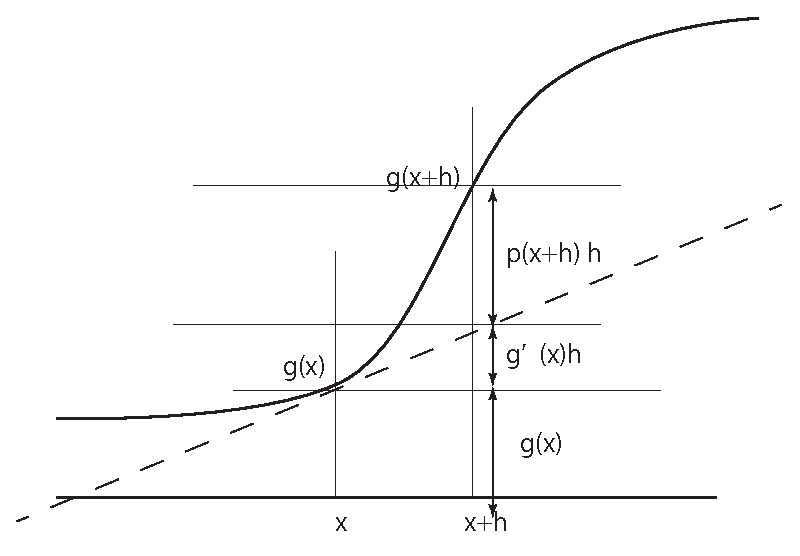
\includegraphics[width=4cm]{calculus5/gosei.eps}
\end{figure}
\end{slide}
\begin{slide}{定理\ref{合成関数}の証明2}
同様に$f(y)$についても微分の誤差を表す関数$q(y) \quad \lim_{u\to 0} q(y+u) = 0$を用い
\begin{equation}
f(y+u) = f(y) + f(y)'u+q(y+u)u \nonumber 
\end{equation}
であり$u = g(x+h) - g(x) = (g'(x) + p(x+h)) h$なので、以下のように求められる。
\begin{eqnarray}
(f(g(x)))' &=& \lim_{h\to 0} \frac{f(y+u) - f(y)}{h}  \nonumber \\
&=& \lim_{h\to 0} \frac{(f'(y) + q(y+u)) u}{h} \nonumber \\
&=& \lim_{h\to 0} \frac{(f'(y) + q(y+u))(g'(x) + p(x+h))\cancel{h}}{\cancel{h}} \nonumber \\
&=& \lim_{h\to 0}(f'(y) + q(y+u))(g'(x) + p(x+h)) = f'(y) g'(x) \nonumber 
\end{eqnarray}
\end{slide}


%%%%%%%%%%%%%%%%%%%%%%%%%%%%%%%%%%%%%%%%%%%%%%%%%%%%%%%%%%%%%%%%%%%%%%%%%%%%%%%%%%%%%%%
%%%%%%%%%%%%%%%%%%%%%%%%%%%%%%%%%%%%%%%%%%%%%%%%%%%%%%%%%%%%%%%%%%%%%%%%%%%%%%%%%%%%%%%


\begin{frame}
\frametitle{合成関数の微分}


$\big((5x^2+3)^9\big)'$を計算することを考える. 
勿論, 展開してから微分しても良いが, 計算が面倒である. \\
\ \\

一方で, $f(y)=y^9$と$g(x)=5x^2+3$を用いて$f(g(x))=(5x^2+3)^9$と書けることから
\begin{align*} 
\big((5x^2+3)^9\big)' &= (y^9)'  \ \ \ \ \ \ \ \ \ \ (y=g(x)\text{とおいた})\\
& =9y^8 \cdot y' \\
&=9(5x^2+3)^8 \cdot 10x \\
&= 90x(5x^2+3)^8. 
\end{align*}
\end{frame}



%%%%%%%%%%%%%%%%%%%%%%%%%%%%%%%%%%%%%%%%%%%%%%%%%%%%%%%%%%%%%%%%%%%%%%%%%%%%%%%%%%%%%%%
%%%%%%%%%%%%%%%%%%%%%%%%%%%%%%%%%%%%%%%%%%%%%%%%%%%%%%%%%%%%%%%%%%%%%%%%%%%%%%%%%%%%%%%


\begin{frame}
\frametitle{合成関数の微分}


$(e^{3x^2+7})'$を計算することを考える. \\
\ \\

$f(y)=e^y$と$g(x)=3x^2+7$を用いて$f(g(x))=e^{3x^2+7}$と書けることから
\begin{align*} 
(e^{3x^2+7})' &= (e^y)'  \ \ \ \ \ \ \ \ \ \ (y=g(x)\text{とおいた})\\
& =e^y \cdot y' \\
&=e^{3x^2+7} \cdot 6x \\
&= 6x e^{3x^2+7}. 
\end{align*}


\end{frame}



%%%%%%%%%%%%%%%%%%%%%%%%%%%%%%%%%%%%%%%%%%%%%%%%%%%%%%%%%%%%%%%%%%%%%%%%%%%%%%%%%%%%%%%
%%%%%%%%%%%%%%%%%%%%%%%%%%%%%%%%%%%%%%%%%%%%%%%%%%%%%%%%%%%%%%%%%%%%%%%%%%%%%%%%%%%%%%%


\begin{frame}
\frametitle{合成関数の微分}


\begin{Prob}
次の関数の導関数を求めよ. 
\begin{enumerate}
\item $(x^2+x+1)^9$, 
\item $\sin^3 x$, 
\item $\cos( x^2)$, 
\item $(x^2+1)^2(2x^3-1)^4$. 
%\item $\cos \frac{1}{x}$, 演習に
%\item $\cos^3(2x+1)$. 
\end{enumerate}
\end{Prob}


\end{frame}




%%%%%%%%%%%%%%%%%%%%%%%%%%%%%%%%%%%%%%%%%%%%%%%%%%%%%%%%%%%%%%%%%%%%%%%%%%%%%%%%%%%%%%%
%%%%%%%%%%%%%%%%%%%%%%%%%%%%%%%%%%%%%%%%%%%%%%%%%%%%%%%%%%%%%%%%%%%%%%%%%%%%%%%%%%%%%%%



\section{一般の指数関数の微分}


\begin{frame}
\frametitle{一般の指数関数の微分}


\begin{Thm} 
$a>0$に関して
$$(a^x)'=a^x \log a$$
\end{Thm}

$a=e^{\log a}$に注意すると
$$
a^x=(e^{\log a})^x=e^{x \log a}
$$
であるから, 
$f(y)=e^y$と$g(x)=x \log a$を用いて$f(g(x))=a^x=e^{x \log a}$と書けることから
\begin{align*} 
(a^x)' &= (e^y)'  =e^y \cdot y' =a^x \log a. 
\end{align*}


\end{frame}


%%%%%%%%%%%%%%%%%%%%%%%%%%%%%%%%%%%%%%%%%%%%%%%%%%%%%%%%%%%%%%%%%%%%%%%%%%%%%%%%%%%%%%%
%%%%%%%%%%%%%%%%%%%%%%%%%%%%%%%%%%%%%%%%%%%%%%%%%%%%%%%%%%%%%%%%%%%%%%%%%%%%%%%%%%%%%%%


\section{対数関数の微分の拡張}

\begin{frame}
\frametitle{対数関数の微分の拡張}

$\log x$の定義域は$x>0$であるが, $\log |x|$を考えることで, 定義域を$x\neq 0$なる実数全体に拡張される. 

 \begin{figure}[htbp]
 \begin{center} 
  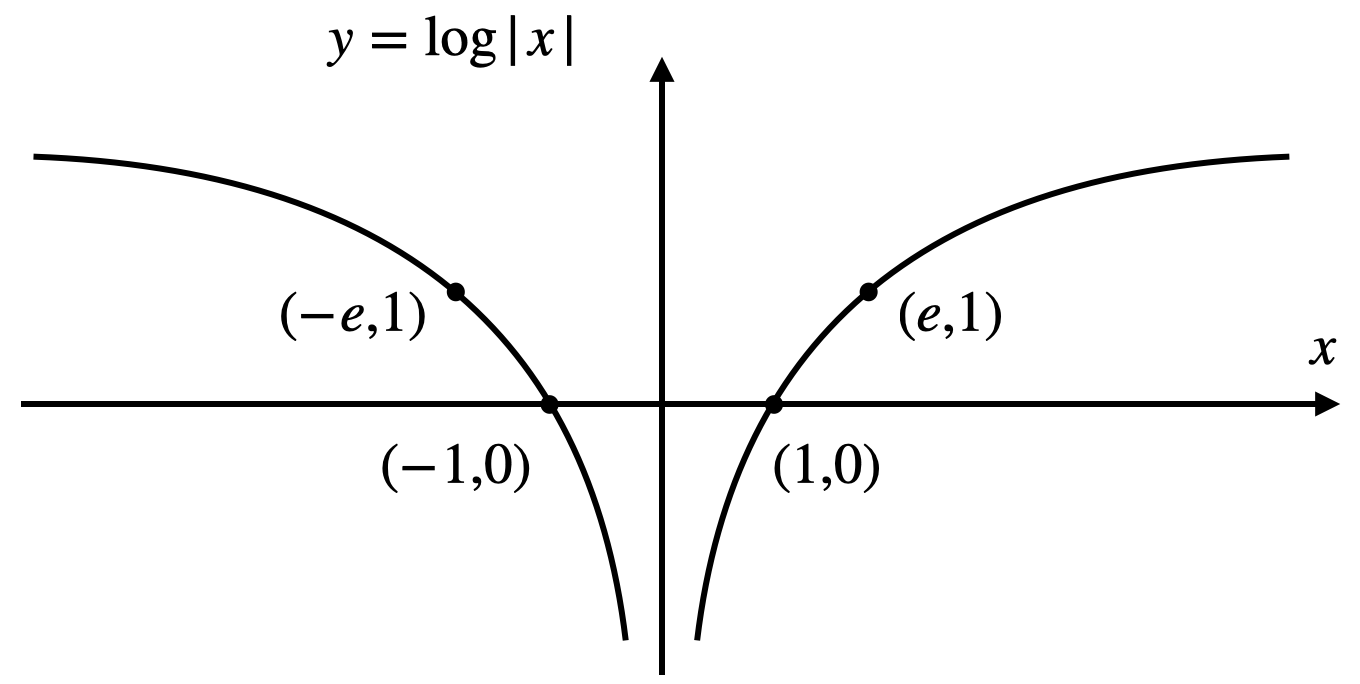
\includegraphics[width=90mm]{calculus5/log_abs.png}
 \end{center}
\end{figure}


\end{frame}


%%%%%%%%%%%%%%%%%%%%%%%%%%%%%%%%%%%%%%%%%%%%%%%%%%%%%%%%%%%%%%%%%%%%%%%%%%%%%%%%%%%%%%%
%%%%%%%%%%%%%%%%%%%%%%%%%%%%%%%%%%%%%%%%%%%%%%%%%%%%%%%%%%%%%%%%%%%%%%%%%%%%%%%%%%%%%%%


\begin{frame}
\frametitle{対数関数の微分の拡張}


\begin{Thm} 
$$(\log |x|)'=\frac{1}{x}$$
\end{Thm}

\begin{itemize}
\item $x>0$の場合
$$
(\log |x|)' = (\log x)'=\frac{1}{x}
$$
\item $x<0$の場合
$$
(\log |x|)' = (\log (-x))'=\frac{1}{-x} \cdot (-1)=\frac{1}{x}. 
$$
\end{itemize}


\end{frame}


%%%%%%%%%%%%%%%%%%%%%%%%%%%%%%%%%%%%%%%%%%%%%%%%%%%%%%%%%%%%%%%%%%%%%%%%%%%%%%%%%%%%%%%
%%%%%%%%%%%%%%%%%%%%%%%%%%%%%%%%%%%%%%%%%%%%%%%%%%%%%%%%%%%%%%%%%%%%%%%%%%%%%%%%%%%%%%%


\section{対数微分}

\begin{frame}
\frametitle{対数微分}



\begin{Thm} \label{対数微分}
微分可能な関数$g(x)$に対して
$$(\log |g(x)|)'=\frac{g'(x)}{g(x)}$$
\end{Thm}

$f(y)=\log |y|$と$g(x)$を用いて$f(g(x))=\log|g(x)|$と書けることから
$$
(\log |g(x)|)'=\frac{1}{g(x)}\cdot g'(x)=\frac{g'(x)}{g(x)}. 
$$
関数の対数を取ってから微分する方法は\underline{対数微分}と呼ばれ, 様々な場面に現れる. 

\end{frame}


%%%%%%%%%%%%%%%%%%%%%%%%%%%%%%%%%%%%%%%%%%%%%%%%%%%%%%%%%%%%%%%%%%%%%%%%%%%%%%%%%%%%%%%
%%%%%%%%%%%%%%%%%%%%%%%%%%%%%%%%%%%%%%%%%%%%%%%%%%%%%%%%%%%%%%%%%%%%%%%%%%%%%%%%%%%%%%%


\begin{frame}
\frametitle{$(x^a)'=ax^{a-1}$}



\begin{Thm} 
$a \in \R$に関して, $x>0$において
$$
(x^a)'=ax^{a-1}.
$$
\end{Thm}
$g(x)=x^a$とすれば
$$
(\log |g(x)|)'= (\log x^a)'= (a \log x)'=\frac{a}{x}. 
$$
定理\ref{対数微分}より
$$
\frac{a}{x}=\frac{g'(x)}{g(x)}=\frac{(x^a)'}{x^a}
$$
であるから
$$
(x^a)'=a x^{a-1}. 
$$
これは対数微分の典型的な応用例. 

\end{frame}


%%%%%%%%%%%%%%%%%%%%%%%%%%%%%%%%%%%%%%%%%%%%%%%%%%%%%%%%%%%%%%%%%%%%%%%%%%%%%%%%%%%%%%%
%%%%%%%%%%%%%%%%%%%%%%%%%%%%%%%%%%%%%%%%%%%%%%%%%%%%%%%%%%%%%%%%%%%%%%%%%%%%%%%%%%%%%%%


\begin{frame}
\frametitle{$(x^a)'=ax^{a-1}$}


具体的に計算すれば
\begin{align*}
(\sqrt{x})' &= (x^{\frac{1}{2}})'=\frac{1}{2}x^{-\frac{1}{2}}= \frac{1}{2 \sqrt{x}}, \\
(\sqrt[3]{x^2})' &= (x^{\frac{2}{3}})'=\frac{2}{3}x^{-\frac{1}{3}}= \frac{2}{3 \sqrt[3]{x}}
\end{align*}

% x^xも対数微分の良い応用例

\end{frame}



%%%%%%%%%%%%%%%%%%%%%%%%%%%%%%%%%%%%%%%%%%%%%%%%%%%%%%%%%%%%%%%%%%%%%%%%%%%%%%%%%%%%%%%
%%%%%%%%%%%%%%%%%%%%%%%%%%%%%%%%%%%%%%%%%%%%%%%%%%%%%%%%%%%%%%%%%%%%%%%%%%%%%%%%%%%%%%%




\section{今日のまとめ}
\begin{frame}
\frametitle{まとめ}   


\begin{enumerate}
\item 三角関数, 指数関数, 対数関数の微分,
\item 合成関数の微分, 対数微分
\end{enumerate} 


\end{frame}
